% Provenance (never printed): see sources/outline_sources.md (Year 3: the
% Rayleigh number; thermal boundary layers; slab pull and ridge push; plumes;
% post-glacial rebound and mantle viscosity). Brief: sources/book5/BRIEFS.md,
% ch. 6. Curves from figdata/bachelor-3/convection_scaling.py (PREM read only),
% gia_relaxation.py and ridge_push.py (on plate_cooling.py). Exercise and
% problem values in the Book 5 scratch calculator calc/ch06.py.
\chapter{Mantelconvectie en plaatdrijvende krachten}\label{ch:b3:mantle-convection}

De kust van Noord-Zweden stijgt ongeveer een centimeter per
jaar uit de zee, tienduizend jaar nadat de ijskap die hem bedekte is weggesmolten; de
kusten van de Hudsonbaai stijgen even snel. Niets duwt ze omhoog behalve de mantel,
die langzaam terugstroomt onder de plek waar het ijs de bodem had ingedrukt. De snelheid
waarmee de bodem terugveert, geeft de viscositeit van de mantel aan, en diezelfde
viscositeit bepaalt hoe snel de mantel convecteert en de platen bewegen. Dit hoofdstuk
vraagt waarom de vaste mantel toch convecteert, hoe snel hij moet stromen om de
warmte van de Aarde te vervoeren, welke krachten de platen in beweging zetten en wat
het herstel van de bodem zegt over de viscositeit van de mantel.
% ledger: vestol19:umea, zhao12:fenno, sella07:gia

\begin{recall}
Viscositeit, de kruipende stroming van een viskeuze vloeistof (de Stokes-vergelijkingen
$\nabla p = \eta\nabla^2\mathbf u$, $\nabla\cdot\mathbf u = 0$), de wet van Stokes
voor een bol, het Reynoldsgetal en het drijfvermogen staan in de universitaire delen van de
natuurkundeboeken. Mantelconvectie en isostatisch herstel kwamen aan bod in de
schoolboeken (leerjaar 12), de rugduw en slabtrek in het deel van leerjaar 11.
De thermische grenslaag, de thermische lithosfeer en de adiabaat van de mantel staan in
Boek~3, in het hoofdstuk over de warmtehuishouding van de Aarde; hotspots,
mantelpluimen en grote magmatische provincies in het hoofdstuk over hotspots.
Het \omterm{def:b3:lithosphere-thermal-models:half-space}{halfruimte-afkoelingsmodel} staat in \cref{ch:b3:lithosphere-thermal-models},
de buiging van de lithosfeer in \cref{ch:b3:gravity-geodesy}, \omterm{def:b3:seismology-imaging:tomography}{seismische
tomografie} in \cref{ch:b3:seismology-imaging}.
\end{recall}

\section{Waarom de mantel convecteert}

De mantel is vast: hij laat S-golven door. Over miljoenen jaren echter kruipt hij
als een vloeistof met een enorme viscositeit, en een laag vloeistof die van onderen
wordt verwarmd en van boven gekoeld, kan in rust blijven, waarbij de warmte door
geleiding wordt afgevoerd, of omslaan. Een klomp warme vloeistof met een grootte van $d$, lichter dan zijn
omgeving met $\rho\alpha\,\Delta T$, stijgt met een snelheid van de orde
$\rho g\alpha\,\Delta T d^2/\eta$; hij verliest zijn warmte door diffusie in een tijd van
de orde $d^2/\kappa$. Kan hij de laag oversteken voordat hij is afgekoeld, dan
slaat de laag om.

\begin{definition}[Rayleighgetal]\label{def:b3:mantle-convection:rayleigh}
Voor een vloeistoflaag met dikte $d$, dichtheid $\rho$, thermische uitzettingscoëfficiënt
$\alpha$, thermische diffusiviteit $\kappa$ en viscositeit $\eta$, onder
invloed van de zwaartekracht $g$, met een temperatuurverschil $\Delta T$ tussen de onderkant en de
bovenkant, is het \emph{Rayleighgetal}\index{Rayleighgetal} gelijk aan
\[
  \mathrm{Ra} = \frac{\rho g\alpha\,\Delta T d^3}{\kappa\eta},
\]
de verhouding van de diffusietijd $d^2/\kappa$ tot de drijvende stijgtijd
$\eta/(\rho g\alpha\,\Delta Td)$.
\end{definition}

\begin{definition}[Kritisch Rayleighgetal]\label{def:b3:mantle-convection:critical}
Het \emph{kritisch Rayleighgetal}\index{kritisch Rayleighgetal}
$\mathrm{Ra}_c$ van een laag is de waarde van het \omterm{def:b3:mantle-convection:rayleigh}{Rayleighgetal} waarboven een
kleine verstoring van de rusttoestand uitgroeit tot convectie, en beneden die waarde
ze wegsterft.
\end{definition}

\begin{proposition}[Het ontstaan van convectie]\label{prop:b3:mantle-convection:onset}
Voor een laag waarvan de boven- en onderkant vrij zijn van schuifspanning en op vaste
temperaturen worden gehouden, groeit een verstoring met horizontaal golfgetal $k$ (in eenheden van $1/d$)
wanneer $\mathrm{Ra} > (\pi^2 + k^2)^3/k^2$. Het minimum van het rechterlid
bij $k = \pi/\sqrt2$, levert
\[
  \mathrm{Ra}_c = \frac{27\pi^4}{4} \approx 657.5,
\]
en de eerste cellen die verschijnen zijn $2\sqrt2\,d$ breed. Tussen starre randen,
$\mathrm{Ra}_c \approx 1708$.
\end{proposition}

\admitted
De lineaire stabiliteitsanalyse erachter, een verstoring van de warmtevergelijking en de
Stokes-vergelijkingen rond de conductieve toestand, staat in de behandeling van
convectie in de natuurkundeboeken; oefening 11 controleert het minimum.

De figuur hieronder toont de convecterende laag. De waarden voor de mantel, met de
diepte van de kern-mantelgrens, $d = \qty{2891}{km}$, de gemiddelde dichtheid van de
mantel, \qty{4476}{kg.m^{-3}}, en $g$ tussen 9.8 en
\qty{10.7}{m.s^{-2}}, alle ontleend aan het seismische aardmodel PREM; $\alpha =
\qty{3.1e-5}{K^{-1}}$ en $\Delta T = \qty{1450}{K}$ uit het plaatmodel
van \cref{ch:b3:lithosphere-thermal-models}; $\kappa = \qty{e-6}{m^2.s^{-1}}$;
en $\eta$ tussen \num{e21} en \qty{e22}{Pa.s} (zie \cref{sec:b3:mantle-convection:gia}),
geven $\mathrm{Ra}$ tussen \num{4.9e6} en \num{4.9e7}, ongeveer zevenduizend tot
zeventigduizend keer de kritische waarde. De mantel kan niet anders dan convecteren.
% ledger: data:prem, honda04:gdh1, delaney86:properties, mitrovica96:haskell, milne04:bifrost

\begin{omfigure}
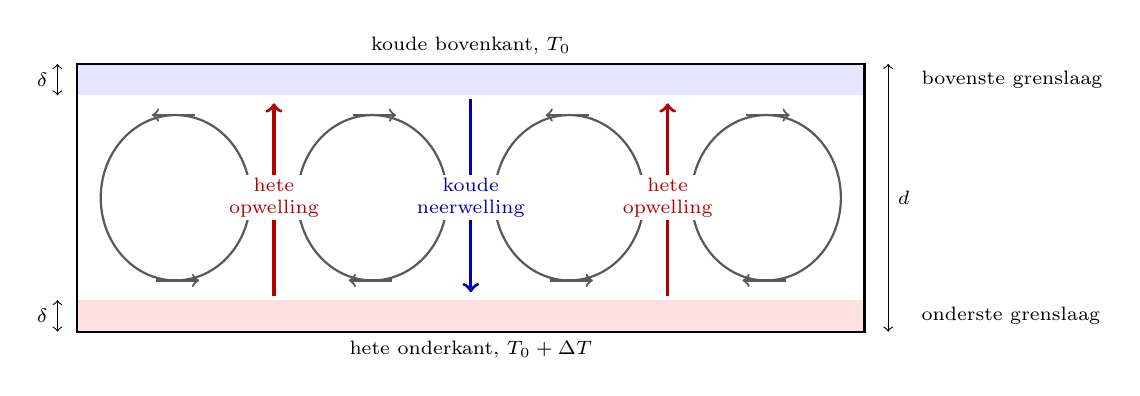
\begin{tikzpicture}[font=\scriptsize, x=1cm, y=1cm]
\fill[blue!10] (0,3.4) rectangle (10,3.0);
\fill[red!12] (0,0) rectangle (10,0.4);
\draw[thick] (0,0) rectangle (10,3.4);
\node[above] at (5,3.4) {koude bovenkant, $T_0$};
\node[below] at (5,0) {hete onderkant, $T_0 + \Delta T$};
\foreach \c/\s in {1.25/1, 3.75/-1, 6.25/1, 8.75/-1} {
  \draw[gray!70!black, thick] (\c,1.7) ellipse[x radius=0.95, y radius=1.05];
  \draw[->, gray!70!black, thick] ({\c+0.25*\s},2.75) -- ({\c-0.3*\s},2.75);
  \draw[->, gray!70!black, thick] ({\c-0.25*\s},0.65) -- ({\c+0.3*\s},0.65);
}
\draw[->, red!70!black, very thick] (2.5,0.45) -- (2.5,2.9);
\draw[->, red!70!black, very thick] (7.5,0.45) -- (7.5,2.9);
\draw[->, blue!70!black, very thick] (5,2.95) -- (5,0.5);
\node[red!70!black, fill=white, inner sep=1pt, align=center] at (2.5,1.7) {hete\\opwelling};
\node[red!70!black, fill=white, inner sep=1pt, align=center] at (7.5,1.7) {hete\\opwelling};
\node[blue!70!black, fill=white, inner sep=1pt, align=center] at (5,1.7) {koude\\neerwelling};
\draw[<->] (10.3,0) -- (10.3,3.4) node[midway, right] {$d$};
\draw[<->] (-0.25,3.0) -- (-0.25,3.4) node[midway, left] {$\delta$};
\draw[<->] (-0.25,0) -- (-0.25,0.4) node[midway, left] {$\delta$};
\node[anchor=west] at (10.6,3.2) {bovenste grenslaag};
\node[anchor=west] at (10.6,0.2) {onderste grenslaag};
\end{tikzpicture}

\par\smallskip{\small Convectie in een laag die van onderen wordt verwarmd en
van boven wordt afgekoeld. Warmte gaat door de dunne grenslagen, met dikte $\delta$, door
geleiding; daartussen transporteert de goed gemengde binnenkant haar door stroming. Koude platen
breken los van de bovenste laag en zinken; warme stijgen op vanaf de
onderste.}\label{fig:b3:mantle-convection:cell}
\end{omfigure}

De mantel wordt ook verwarmd van binnenuit, door het verval van radioactieve elementen,
en van onderen, door de kern. Een laag die alleen van binnenuit wordt verwarmd, heeft geen hete
grenslaag aan haar basis: de stroming wordt aangedreven door koude platen die vanaf de
bovenkant zinken, terwijl de opstijgende stroming een brede, passieve terugstroom is. Slabs zijn zulke platen, en
pluimen hebben de warmte van de kern nodig.

\section{Grenslagen en de sterkte van de convectie}

\begin{definition}[Nusseltgetal]\label{def:b3:mantle-convection:nusselt}
Het \emph{Nusseltgetal}\index{Nusseltgetal} van een convecterende laag is de
warmtestroom erdoor gedeeld door de warmtestroom die geleiding alleen over
dezelfde laag zou transporteren, $\mathrm{Nu} = q\,d/(k\,\Delta T)$.
\end{definition}

\begin{theorem}[Grenslaagschaling van convectie]\label{thm:b3:mantle-convection:scaling}
In een laag die convecteert bij $\mathrm{Ra} \gg \mathrm{Ra}_c$, als elke thermische
grenslaag groeit tot haar eigen \omterm{def:b3:mantle-convection:rayleigh}{Rayleighgetal}, opgebouwd met haar dikte
$\delta$ en het temperatuurverschil $\Delta T/2$ erover, bereikt
$\mathrm{Ra}_c$, dan geldt
\[
  \delta = d\Bigl(\frac{2\mathrm{Ra}_c}{\mathrm{Ra}}\Bigr)^{1/3},\qquad
  \mathrm{Nu} = \frac12\Bigl(\frac{\mathrm{Ra}}{2\mathrm{Ra}_c}\Bigr)^{1/3},
  \qquad
  u = \frac\kappa d\Bigl(\frac{\mathrm{Ra}}{2\mathrm{Ra}_c}\Bigr)^{2/3},
\]
waarbij $u$ de snelheidsschaal van de stroming is, gedefinieerd door te eisen dat de
laag groeit tot $\delta$ terwijl de vloeistof de cel doorkruist. Dit is de
\emph{grenslaagschaling van convectie}\index{grenslaagschaling van convectie}.
\end{theorem}

\begin{proof}
Het inwendige is goed gemengd, op de gemiddelde temperatuur, dus draagt elke grenslaag
de helft van $\Delta T$. Haar \omterm{def:b3:mantle-convection:rayleigh}{Rayleighgetal} is $\rho g\alpha(\Delta T/2)
\delta^3/(\kappa\eta) = \mathrm{Ra}\,(\delta/d)^3/2$; als je dit gelijkstelt aan
$\mathrm{Ra}_c$, volgt $\delta$. De warmtestroom wordt door de laag geleid,
$q = k(\Delta T/2)/\delta$, dus $\mathrm{Nu} = qd/(k\Delta T) = d/(2\delta)$.
Een grenslaag groeit door diffusie tot de dikte $\delta$ in een tijd
$\delta^2/\kappa$; het bovenste fluïdum doorkruist de cel, met een breedte van de orde
$d$, in een tijd $d/u$. Door de twee tijden gelijk te stellen, volgt $u = \kappa d/\delta^2 =
(\kappa/d)(d/\delta)^2$.
\end{proof}

De warmtestroom groeit alleen als de derdemachtswortel van $\mathrm{Ra}$: een honderd keer
lagere viscositeit geeft minder dan vijf keer zoveel warmte. Met de
$\mathrm{Ra} = \num{4.9e7}$ van de mantel geeft de schaling $\delta \approx \qty{87}{km}$,
$\mathrm{Nu} \approx 17$, een warmtestroom van $\mathrm{Nu}\,k\Delta T/d \approx
\qty{26}{mW.m^{-2}}$ met $k = \qty{3.1}{W.m^{-1}.K^{-1}}$, en $u \approx
\qty{1.2}{cm/yr}$ (figuur hieronder). De grenslaag is even dik als de
oceanische plaat van \cref{ch:b3:lithosphere-thermal-models}, \qty{95}{km}; de
quadratisch gemiddelde snelheden van de huidige platen lopen van \qty{1.1}{cm/yr}
(Zuid-Amerika) tot \qty{7.5}{cm/yr} (Cocos), \qty{4.4}{cm/yr} voor de hele
lithosfeer. De gemiddelde warmtestroom van de Aarde, \qty{92}{mW.m^{-2}}, is drie tot vier
keer die van de schaling: de warmte die in de mantel zelf wordt geproduceerd, die een laag
die van onderen wordt verwarmd weglaat, en de constanten van de orde één die de schaling
negeert, dragen beide bij. Voor een wet met één invoer kloppen de ordes van grootte:
platen zijn de bovenste grenslaag van een mantel met $\mathrm{Ra}
\sim 10^7$.
% ledger: nnr56:rms, b2dd10:continents, honda04:gdh1

\begin{omfigure}
\begin{tikzpicture}
\begin{groupplot}[group style={group size=1 by 2, vertical sep=2.5cm},
  omrecord, width=0.86\linewidth, height=0.40\linewidth, xmode=log, ymode=log,
  xmin=100, xmax=1e10, xlabel={Rayleighgetal $\mathrm{Ra}$}]
\nextgroupplot[ylabel={Nusseltgetal}, ymin=0.3, ymax=300,
  title={(a) warmtestroom, in eenheden van de geleidingsstroom}, title style={font=\small}]
% computed in figdata/bachelor-3/convection_scaling.py; ledger: data:prem, honda04:gdh1
\addplot[omDef, thick] table[x=ra, y=nu] {figdata/out/bachelor-3-convection_scaling-conduction.dat};
\addplot[red!70!black, thick] table[x=ra, y=nu] {figdata/out/bachelor-3-convection_scaling-scaling.dat};
\addplot[gray, densely dashed, unbounded coords=jump] table[x=ra, y=y] {figdata/out/bachelor-3-convection_scaling-band.dat};
\draw[gray, densely dotted] (axis cs:657.5,0.3) -- (axis cs:657.5,1);
\node[font=\scriptsize, anchor=west] at (axis cs:700,0.45) {$\mathrm{Ra}_c$};
\node[font=\scriptsize, anchor=south west, omDef] at (axis cs:115,1.08) {geleiding};
\node[font=\scriptsize, anchor=north west, red!70!black] at (axis cs:3e4,0.95) {$\tfrac12(\mathrm{Ra}/2\mathrm{Ra}_c)^{1/3}$};
\node[font=\scriptsize, fill=white, inner sep=1pt] at (axis cs:1.55e7,120) {mantel};
\nextgroupplot[ylabel={snelheid (\unit{cm/yr})}, ymin=1e-3, ymax=100,
  title={(b) snelheidsschaal voor $d = \qty{2891}{km}$}, title style={font=\small}]
\addplot[red!70!black, thick] table[x=ra, y=u] {figdata/out/bachelor-3-convection_scaling-scaling.dat};
\addplot[gray, densely dashed, unbounded coords=jump] table[x=ra, y=y] {figdata/out/bachelor-3-convection_scaling-band.dat};
\addplot[blue!70, thick, dash dot, unbounded coords=jump] table[x=ra, y=u] {figdata/out/bachelor-3-convection_scaling-plates.dat};
\node[font=\scriptsize, anchor=south west, blue!60!black] at (axis cs:150,7.6) {snelste plaat};
\node[font=\scriptsize, anchor=north west, blue!60!black] at (axis cs:150,1.0) {traagste plaat};
\node[font=\scriptsize, fill=white, inner sep=1pt] at (axis cs:1.55e7,0.004) {mantel};
\end{groupplot}
\end{tikzpicture}

\par\smallskip{\small Convectieschaling. (a) Onder $\mathrm{Ra}_c$ de laag
geleidt ($\mathrm{Nu} = 1$); ver daarboven de grenslaagwet, getekend
vanaf $\mathrm{Ra} = 16\,\mathrm{Ra}_c \approx \num{1.1e4}$, waar die $\mathrm{Nu} = 1$ geeft (ertussenin
begint convectie geleidelijk). (b) De snelheidsschaal voor
de diepte van de mantel en $\kappa = \qty{e-6}{m^2.s^{-1}}$, met het
bereik van de huidige plaatsnelheden (streep-stip). De gestreepte lijnen begrenzen het
\omterm{def:b3:mantle-convection:rayleigh}{Rayleighgetal} van de mantel voor viscositeiten van \num{e22} en \qty{e21}{Pa.s}.}\label{fig:b3:mantle-convection:scaling}
\end{omfigure}

\section{De krachten op een plaat}

Een plaat beweegt met een stationaire snelheid: de krachten erop heffen elkaar op. Drie krachten drijven haar aan of
werken haar tegen, aan haar randen en aan haar basis (figuur hieronder). De kracht die de
zinkende slab op haar plaat uitoefent, slabtrek, komt voort uit het overschot aan dichtheid van
een koude slab in de warmere mantel. Rugduw, de duw van de hoge, hete rug
op de koelere plaat ernaast, volgt uit het halfruimtemodel van
\cref{ch:b3:lithosphere-thermal-models}.

\begin{omfigure}
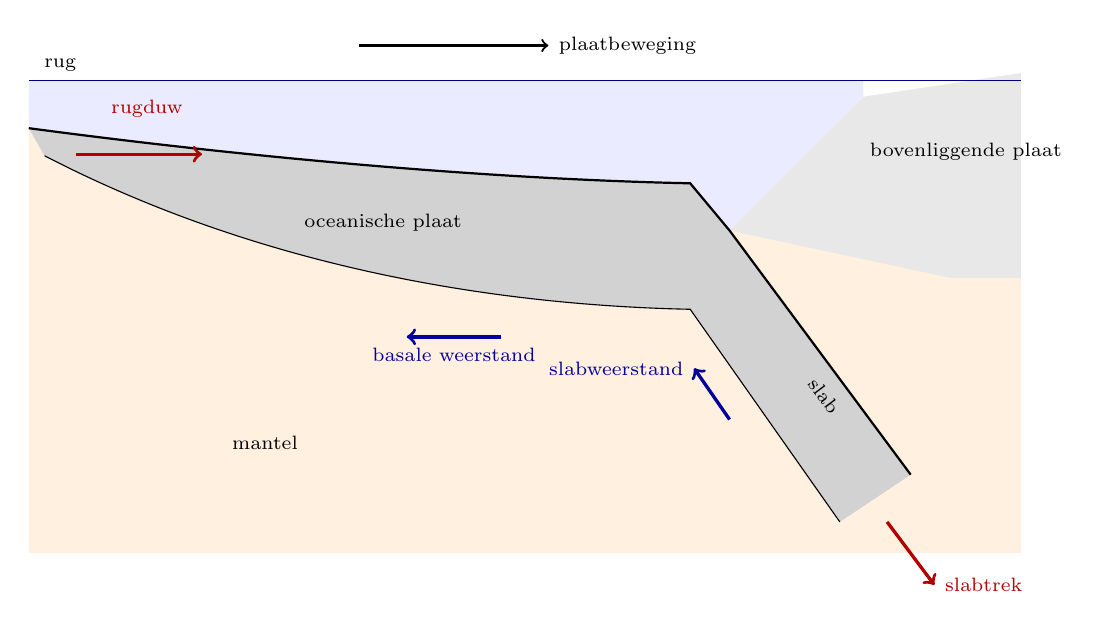
\begin{tikzpicture}[font=\scriptsize, x=1cm, y=1cm]
\fill[orange!12] (0,-0.6) rectangle (12.6,-6.0);
\fill[blue!8] (0,0) -- (0,-0.6) .. controls (3,-1.0) and (6,-1.25) .. (8.4,-1.3) -- (8.9,-1.9) -- (10.6,-0.2) -- (10.6,0) -- cycle;
\fill[gray!35] (0,-0.6) .. controls (3,-1.0) and (6,-1.25) .. (8.4,-1.3) -- (8.9,-1.9) -- (11.2,-5.0) -- (10.3,-5.6) -- (8.4,-2.9) .. controls (6,-2.85) and (3,-2.4) .. (0.2,-0.95) -- cycle;
\fill[gray!18] (10.6,-0.2) -- (12.6,0.1) -- (12.6,-2.5) -- (11.7,-2.5) -- (8.9,-1.9) -- cycle;
\draw[thick] (0,-0.6) .. controls (3,-1.0) and (6,-1.25) .. (8.4,-1.3) -- (8.9,-1.9) -- (11.2,-5.0);
\draw (0.2,-0.95) .. controls (3,-2.4) and (6,-2.85) .. (8.4,-2.9) -- (10.3,-5.6);
\draw[blue!50!black] (0,0) -- (12.6,0);
\node at (0.4,0.2) {rug};
\node at (4.5,-1.8) {oceanische plaat};
\node at (11.9,-0.9) {bovenliggende plaat};
\node[rotate=-53] at (10.1,-4.0) {slab};
\node at (3,-4.6) {mantel};
\draw[->, very thick, red!70!black] (0.6,-0.93) -- (2.2,-0.93);
\node[red!70!black] at (1.5,-0.35) {rugduw};
\draw[->, very thick, red!70!black] (10.9,-5.6) -- (11.5,-6.4) node[right] {slabtrek};
\draw[->, very thick, blue!60!black] (6.0,-3.25) -- (4.8,-3.25) node[below, pos=0.5] {basale weerstand};
\draw[->, very thick, blue!60!black] (8.9,-4.3) -- (8.45,-3.65) node[left] {slabweerstand};
\draw[->, thick] (4.2,0.45) -- (6.6,0.45) node[right] {plaatbeweging};
\end{tikzpicture}

\par\smallskip{\small De krachten op een oceanische plaat: rugduw en slabtrek
drijven haar aan (rood); de \omterm{def:b3:mantle-convection:basal-drag}{basale weerstand} aan haar basis, waar de plaat sneller beweegt dan de mantel
eronder, en de viskeuze weerstand van de mantel tegen de zinkende slab werken
haar tegen (blauw).}\label{fig:b3:mantle-convection:forces}
\end{omfigure}

\begin{proposition}[Rugduwkracht]\label{prop:b3:mantle-convection:ridge-push}
In het \omterm{def:b3:lithosphere-thermal-models:half-space}{halfruimte-afkoelingsmodel}, met manteltemperatuur $T_m$,
oppervlaktetemperatuur $T_0$ en isostatische compensatie, de horizontale kracht per eenheid
van rug die de kolom bij de rug op de plaat van ouderdom $t$ uitoefent,
de \emph{rugduwkracht}\index{rugduwkracht}, is
\[
  F_{rp} = g\rho_m\alpha(T_m - T_0)\kappa t\Bigl[1 + \frac{2\rho_m\alpha(T_m
  - T_0)}{\pi(\rho_m - \rho_w)}\Bigr].
\]
\end{proposition}

\begin{proof}
Laat $y$ de diepte onder de zeebodem bij de rug zijn, $w$ de subsidentie van
de bodem van ouderdom $t$, $\theta(z) = T_m - T(z)$ het temperatuurtekort op de
diepte $z = y - w$ in de plaat, en $\Theta(z) = \int_0^z\theta$. Bij de rug
bevat de kolom mantel met dichtheid $\rho_m$ vanaf $y = 0$; de oude kolom bevat
water tot $w$, daarna plaat met dichtheid $\rho_m(1 + \alpha\theta)$. De
litostatische drukken verschillen met $P_r - P_t = (\rho_m - \rho_w)gy$ voor $y < w$,
en daaronder,
\[
  P_r - P_t = (\rho_m - \rho_w)gw - \rho_mg\alpha\,\Theta(z)
  = \rho_mg\alpha\bigl(\Theta(\infty) - \Theta(z)\bigr),
\]
volgens de isostasie, $(\rho_m - \rho_w)w = \rho_m\alpha\Theta(\infty)$. De kracht is de
integraal van het drukverschil over de diepte; door het tweede deel partieel
te integreren,
\[
  F_{rp} = \tfrac12(\rho_m - \rho_w)gw^2 + \rho_mg\alpha\int_0^\infty
  z\,\theta(z)\,\mathrm dz .
\]
Voor het halfruimte, $\theta = (T_m - T_0)\operatorname{erfc}(z/2\sqrt{\kappa
t})$ en $\int_0^\infty x\operatorname{erfc}x\,\mathrm dx = 1/4$, dus de
integraal is $(T_m - T_0)\kappa t$; en $w = 2\rho_m\alpha(T_m -
T_0)\sqrt{\kappa t/\pi}/(\rho_m - \rho_w)$. Het optellen van de twee termen levert de
formule op.
\end{proof}

Rugduw neemt lineair toe met de ouderdom: het is geen duw aan de as maar een
drukgradiënt die over de hele afkoelende plaat is verdeeld. Met de waarden van
\cref{ch:b3:lithosphere-thermal-models}, de term tussen haakjes is 1.04 en $F_{rp} =
\qty{3.8e12}{N.m^{-1}}$ bij \qty{100}{Myr}. In het plaatmodel houdt ze op met groeien
met de diepte, op ongeveer \qty{2.3e12}{N.m^{-1}} (figuur hieronder). Slabtrek is
groter: een slab van \qty{95}{km} dikte, gemiddeld $(T_m - T_0)/2$ kouder dan de
mantel, en dus dichter met $\rho_m\alpha(T_m - T_0)/2 \approx
\qty{74}{kg.m^{-3}}$, die tot \qty{670}{km} diep hangt, weegt
\qty{4.6e13}{N.m^{-1}} meer dan de mantel die hij verplaatst, twaalf keer de
rugduw. Een groot deel van dat gewicht gaat op aan de viskeuze mantel die het zinken van de
slab tegenwerkt, en slechts een deel bereikt de plaat.
% ledger: honda04:gdh1, data:prem

\begin{omfigure}
\begin{tikzpicture}
\begin{axis}[omrecord, width=0.8\linewidth, height=0.42\linewidth,
  xmin=0, xmax=160, ymin=0, ymax=6.5, xlabel={ouderdom van de zeebodem (Myr)},
  ylabel={$F_{rp}$ (\qty{e12}{N.m^{-1}})},
  legend cell align=left,
  legend style={font=\scriptsize, at={(0.03,0.97)}, anchor=north west}]
% computed in figdata/bachelor-3/ridge_push.py; ledger: honda04:gdh1
\addplot[omDef, thick] table[x=t, y=hs] {figdata/out/bachelor-3-ridge_push-force.dat};
\addlegendentry{halfruimte}
\addplot[red!70!black, thick, densely dashed] table[x=t, y=pl] {figdata/out/bachelor-3-ridge_push-force.dat};
\addlegendentry{plaat, $L = \qty{95}{km}$}
\end{axis}
\end{tikzpicture}

\par\smallskip{\small \omterm{prop:b3:mantle-convection:ridge-push}{Rugduwkracht} als functie van de ouderdom van de plaat, uit de
twee afkoelingsmodellen van \cref{ch:b3:lithosphere-thermal-models}, door numerieke
integratie van het drukverschil (de halfruimtecurve is de gesloten
vorm van de propositie).}\label{fig:b3:mantle-convection:ridge-push}
\end{omfigure}

\begin{definition}[Basale weerstand]\label{def:b3:mantle-convection:basal-drag}
\emph{Basale weerstand}\index{basale weerstand} is de schuifkracht per oppervlakte-eenheid die de
mantel onder een plaat uitoefent op de basis van de plaat. Voor een plaat die met $u$ beweegt
over een laag met dikte $h$ en viscositeit $\eta$ waarvan de basis stilstaat, bedraagt de
weerstand $\eta u/h$, tegengesteld aan de beweging; zij drijft de plaat aan waar de mantel
eronder sneller beweegt dan de plaat.
\end{definition}

Welke krachten ertoe doen, valt af te lezen aan de platen zelf. De koppelbalans
op elke plaat, aangepast aan de plaatbewegingen, zegt dat de krachten die op de
zinkende slab werken de snelheid van oceanische platen bepalen en ongeveer tien keer
sterker zijn dan alle andere, en dat de weerstand aan de basis groter is onder
continenten dan onder oceanen. De snelheden stemmen overeen: de snelste platen, Cocos met
\qty{75}{mm/yr}, Nazca met 70 en de Pacifische plaat met \qty{66}{mm/yr}, zijn oceanische
platen waarvan de randen in lange greppels zinken; de traagste dragen grote continenten,
Eurazië met 23, Noord-Amerika met 20, Zuid-Amerika met \qty{11}{mm/yr}.
% ledger: fu75:slab-pull, nnr56:rms

\section{Pluimen}

Warme platen die van de basis van de mantel opstijgen, verzamelen zich tot kolommen:
de mantelpluimen uit Boek~3, met een grote kop en een dunne staart (figuur hieronder).
De opwelling van een hotspot, een brede verhoging van de zeebodem rond en stroomafwaarts van
de vulkanen, meet hoeveel drijfvermogen de pluim aanvoert.

\begin{definition}[Drijfvermogenflux van de pluim]\label{def:b3:mantle-convection:buoyancy-flux}
De \emph{drijfvermogenflux van de pluim}\index{drijfvermogenflux van de pluim} $B$ is het massatekort,
ten opzichte van de omringende mantel, dat een pluim per
tijdseenheid omhoog voert; voor een pluim met volumeflux $Q_v$ en temperatuuroverschot $\Delta T$,
geldt $B = \rho\alpha\,\Delta T\,Q_v$.
\end{definition}

\begin{proposition}[Drijfvermogenflux uit een opwelling]\label{prop:b3:mantle-convection:swell}
Als een plaat die met snelheid $u$ over een pluim beweegt, een opwelling met
dwarsdoorsnede $A$ dwars op het spoor meevoert, die isostatisch wordt gedragen door het
pluimmateriaal eronder, dan is de \omterm{def:b3:mantle-convection:buoyancy-flux}{drijfvermogenflux van de pluim}
\[
  B = (\rho_m - \rho_w)\,A\,u .
\]
\end{proposition}

\begin{proof}
Door isostasie wordt een plak opwelling van eenheidslengte langs het spoor, die de zeebodem
over het oppervlak $A$ van de dwarsdoorsnede optilt en water door gesteente vervangt,
wordt gedragen door een massatekort $(\rho_m - \rho_w)A$ in de kolom eronder.
De plaat voert de plak weg met snelheid $u$, dus in de stationaire toestand moet de
pluim het tekort leveren voor een lengte $u$ van nieuwe opwelling per tijdseenheid.
\end{proof}

Uit de dwarsdoorsneden van de opwellingen varieert de drijfvermogenflux van hotspots over
een factor twintig: Hawaï, de grootste, \qty{8.7}{Mg/s}; IJsland
\qty{1.4}{Mg/s}; 37 hotspots samen ongeveer \qty{50}{Mg/s}. Elke kilogram
drijfvermogen komt overeen met $c_p/\alpha$ joule overtollige warmte, dus de warmtestroom is $c_pB/\alpha$;
met $c_p = k/(\rho_m\kappa) = \qty{1170}{J.kg^{-1}.K^{-1}}$ en $\alpha =
\qty{3.1e-5}{K^{-1}}$, dragen de 37 hotspots ongeveer \qty{1.9}{TW}, of
\qty{3.7}{mW.m^{-2}} verdeeld over het aardoppervlak van \qty{5.1e14}{m^2}, dicht bij de
\qty{4}{mW.m^{-2}} gepubliceerd bij de fluxen: enkele procenten van de
\qty{47}{TW} die de Aarde verliest. Pluimen zijn de kleine partner van het
warmtebudget; de platen dragen de rest.
% ledger: sleep90:flux, b2dd10:half-space, honda04:gdh1

\begin{omfigure}
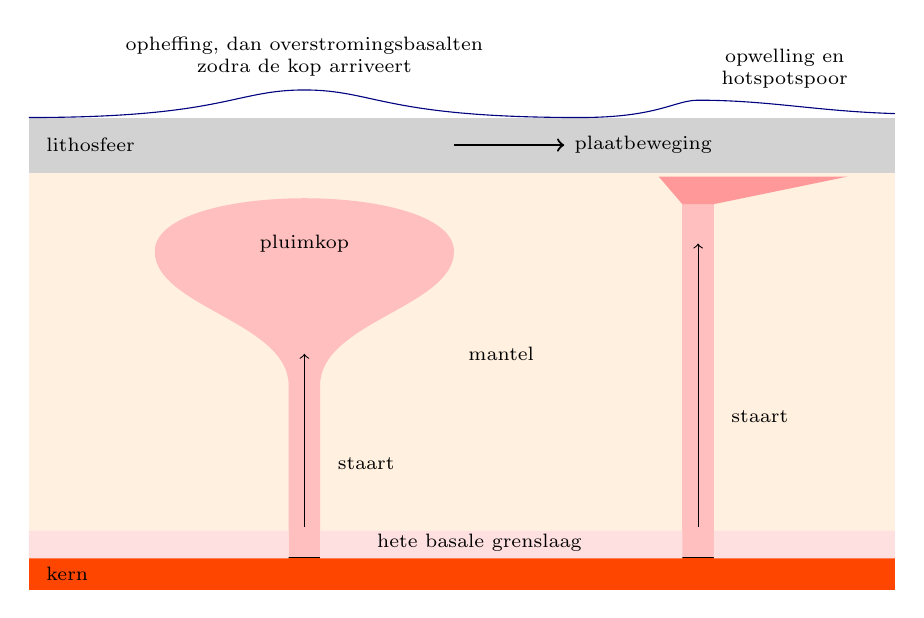
\begin{tikzpicture}[font=\scriptsize, x=1cm, y=1cm]
\fill[orange!12] (0,0) rectangle (11,-5.6);
\fill[gray!35] (0,0) -- (11,0) -- (11,-0.7) -- (0,-0.7) -- cycle;
\fill[red!25] (3.3,-5.6) -- (3.3,-3.4) .. controls (3.3,-2.6) and (1.6,-2.4) .. (1.6,-1.7)
  .. controls (1.6,-0.8) and (5.4,-0.8) .. (5.4,-1.7) .. controls (5.4,-2.4) and (3.7,-2.6) .. (3.7,-3.4) -- (3.7,-5.6) -- cycle;
\fill[red!25] (8.3,-5.6) -- (8.3,-0.75) -- (8.7,-0.75) -- (8.7,-5.6) -- cycle;
\fill[red!40] (8.0,-0.75) -- (8.3,-1.1) -- (8.7,-1.1) -- (10.4,-0.75) -- cycle;
\draw[thick] (0,-5.6) -- (11,-5.6);
\fill[red!45!orange] (0,-5.6) rectangle (11,-6.0);
\fill[red!12] (0,-5.6) rectangle (3.3,-5.25) (3.7,-5.6) rectangle (8.3,-5.25) (8.7,-5.6) rectangle (11,-5.25);
\node[anchor=west] at (0.1,-5.8) {kern};
\node at (3.5,-1.6) {pluimkop};
\node[anchor=west] at (3.8,-4.4) {staart};
\node[anchor=west] at (8.8,-3.8) {staart};
\node[anchor=west] at (0.1,-0.35) {lithosfeer};
\node at (6.0,-3.0) {mantel};
\draw[->] (3.5,-5.2) -- (3.5,-3.0);
\draw[->] (8.5,-5.2) -- (8.5,-1.6);
\draw[->, thick] (5.4,-0.35) -- (6.8,-0.35) node[right] {plaatbeweging};
\draw[blue!50!black] (0,0) .. controls (2.5,0) and (2.6,0.35) .. (3.5,0.35) .. controls (4.4,0.35) and (4.5,0) .. (7,0) .. controls (8,0) and (8.2,0.22) .. (8.5,0.22) .. controls (9.4,0.22) and (10,0.08) .. (11,0.05);
\node[above, align=center] at (3.5,0.4) {opheffing, dan overstromingsbasalten\\zodra de kop arriveert};
\node[above, align=center] at (9.6,0.25) {opwelling en\\hotspotspoor};
\node[anchor=west] at (4.3,-5.4) {hete basale grenslaag};
\end{tikzpicture}

\par\smallskip{\small Een jonge pluim (links) stijgt op als een grote kop, gevoed door een dunne
staart; wanneer de kop zich onder de lithosfeer verspreidt, stijgt het oppervlak en kunnen
overstromingsbasalten uitbarsten. Een oudere pluim (rechts) is een staart onder een bewegende plaat,
die een opwelling en een hotspotspoor voedt. Niet op
schaal.}\label{fig:b3:mantle-convection:plume}
\end{omfigure}

Een pluimkop is een bol van drijvende mantel die door de viskeuze mantel omhoog stijgt:
De Stokes-wet uit de natuurkunde, $v = 2\Delta\rho\,ga^2/(9\eta)$, geeft de snelheid
in grootteorde, een fractie van een meter per jaar voor een kop van enkele honderden
kilometers in doorsnede (opgave 8), zodat ze de mantel in miljoenen jaren doorkruist.

\section{Glaciaal-isostatische aanpassing en de mantelviscositeit}\label{sec:b3:mantle-convection:gia}

\begin{definition}[Glaciaal-isostatische aanpassing, mantelviscositeit]\label{def:b3:mantle-convection:gia}
\emph{glaciaal-isostatische aanpassing}\index{glaciaal-isostatische aanpassing} (GIA)
is de langzame vervorming van de vaste Aarde, en de verandering van haar zwaartekrachtveld
en van het zeeniveau, terwijl ze na het groeien of smelten van een
ijskap terugkeert naar isostatisch evenwicht. De \emph{mantelviscositeit}\index{mantelviscositeit}
is de effectieve viscositeit $\eta$ die het langzame, gelijkmatige kruip van de
mantel koppelt aan de spanningen die het aandrijven, over tijdschalen van duizenden jaren en langer.
\end{definition}

Wanneer een ijskap smelt, is de inzinking die hij achterlaat uit isostatisch
evenwicht: eronder is de druk in de mantel lager dan eromheen, en
stroomt mantelmateriaal toe om de bodem weer op te tillen. Vandaag stijgt de kust van de Botnische Golf
met maximaal \qty{10.3}{mm/yr}, bij Umeå; de Hudsonbaai met ongeveer
\qty{10}{mm/yr}, waar het ijs het dikst was, terwijl het land ten zuiden van de
Grote Meren daalt met 1 tot \qty{2}{mm/yr}, doordat de bult die het ijs eromheen had opgestuwd
daalt. Aan de kusten staan oude strandlijnen nu boven de zee, de
opgeheven stranden van het veldkader hieronder.
% ledger: vestol19:umea, sella07:gia

\begin{theorem}[Relaxatie van een viskeuze halfruimte]\label{thm:b3:mantle-convection:relaxation}
Een inzinking $w(x, t) = w_m(t)\cos(2\pi x/\lambda)$ van het oppervlak van een
halfruimte met uniforme viscositeit $\eta$ en dichtheid $\rho$, zonder belasting achtergelaten,
vervalt volgens $w_m(t) = w_m(0)e^{-t/\tau}$ met
\[
  \tau = \frac{4\pi\eta}{\rho g\lambda} .
\]
\end{theorem}

\begin{proof}
Neem $z$ naar beneden, $k = 2\pi/\lambda$, en zoek naar een Stokesstroming die
met de diepte afneemt, met verticale snelheid (naar beneden) $v = (C + Dkz)e^{-kz}\cos kx$.
Uit de onsamendrukbaarheid volgt de horizontale snelheid $u = -(D - C - Dkz)e^{-kz}\sin
kx$. Deze functies voldoen aan $\nabla^4 = 0$, zoals elke Stokesstroming in twee
dimensies doet. Het vrije oppervlak draagt geen schuifspanning: $\partial u/\partial
z + \partial v/\partial x = 2k(D - C)\sin kx = 0$ bij $z = 0$, dus $D = C$, en
\[
  v = C(1 + kz)e^{-kz}\cos kx,\quad u = Ckze^{-kz}\sin kx,\quad
  p = 2\eta Cke^{-kz}\cos kx,
\]
waarbij de druk volgt uit $\partial p/\partial x = \eta\nabla^2u = -2\eta
Ck^2e^{-kz}\sin kx$ (en $\partial p/\partial z = \eta\nabla^2v$ klopt). Aan het
oppervlak geldt $\partial v/\partial z = 0$, dus is de normaalspanning daar $-p$. Onder
een inzinking $w$ verlaagt het gewicht van het ontbrekende gesteente de druk met $\rho
gw$: $p(0) = -\rho gw$, dus $2\eta Ck = -\rho gw_m$. Het oppervlak beweegt mee met de
vloeistof: $\mathrm dw_m/\mathrm dt = v(0) = C = -\rho gw_m/(2\eta k)$, en de
oplossing hiervan vervalt met $\tau = 2\eta k/(\rho g) = 4\pi\eta/(\rho g\lambda)$.
\end{proof}

\begin{definition}[Isostatische relaxatietijd]\label{def:b3:mantle-convection:relaxation-time}
De \emph{isostatische relaxatietijd}\index{isostatische relaxatietijd} $\tau$ van
een belasting met horizontale schaal $\lambda$ is de tijd waarin de afwijking van
het isostatisch evenwicht met een factor $e$ afneemt.
\end{definition}

Een uniforme halfruimte herstelt brede inzakkingen sneller dan smalle, en de
stroming onder een belasting met golflengte $\lambda$ neemt met de diepte af als $e^{-kz}$, over
een diepte van $\lambda/2\pi$: een grote ijskap roert de mantel diep om, een klein meer
alleen de bovenkant. Voor een inzakking van \qty{3000}{km} breed en $\eta =
\qty{e21}{Pa.s}$, met $\rho = \qty{3300}{kg.m^{-3}}$, $\tau = \qty{4.1}{kyr}$
(figuur hieronder): na tienduizend jaar is $e^{-2.4} = \qty{9}{\percent}$ van de
inzakking over, en omdat $\dot w = -w/\tau$, betekent een opheffing van
\qty{10}{mm/yr} dat nog ongeveer \qty{40}{m} stijging te gaan is.

\begin{omfigure}
\begin{tikzpicture}
\begin{groupplot}[group style={group size=1 by 2, vertical sep=2.5cm},
  omrecord, width=0.86\linewidth, height=0.38\linewidth]
\nextgroupplot[xmin=0, xmax=20, ymin=0, ymax=1.05, xlabel={tijd sinds het ijs smolt (kyr)},
  ylabel={$w_m(t)/w_m(0)$}, title={(a) verval van een inzakking van \qty{3000}{km} breed},
  title style={font=\small}, legend style={font=\scriptsize, at={(0.98,0.97)}, anchor=north east}]
% computed in figdata/bachelor-3/gia_relaxation.py; ledger: mitrovica96:haskell, milne04:bifrost
\addplot[red!70!black, thick, densely dashed] table[x=t, y=f20] {figdata/out/bachelor-3-gia_relaxation-decay.dat};
\addlegendentry{$\eta = \qty{e20}{Pa.s}$}
\addplot[omDef, thick] table[x=t, y=f21] {figdata/out/bachelor-3-gia_relaxation-decay.dat};
\addlegendentry{$\eta = \qty{e21}{Pa.s}$}
\addplot[black, thick, densely dotted] table[x=t, y=f22] {figdata/out/bachelor-3-gia_relaxation-decay.dat};
\addlegendentry{$\eta = \qty{e22}{Pa.s}$}
\nextgroupplot[xmode=log, ymode=log, xmin=100, xmax=1e4, ymin=0.01, ymax=1000,
  xlabel={golflengte $\lambda$ (km)}, ylabel={$\tau$ (kyr)},
  title={(b) relaxatietijd tegen golflengte}, title style={font=\small}]
\addplot[red!70!black, thick, densely dashed] table[x=lam, y=t20] {figdata/out/bachelor-3-gia_relaxation-tau.dat};
\addplot[omDef, thick] table[x=lam, y=t21] {figdata/out/bachelor-3-gia_relaxation-tau.dat};
\addplot[black, thick, densely dotted] table[x=lam, y=t22] {figdata/out/bachelor-3-gia_relaxation-tau.dat};
\end{groupplot}
\end{tikzpicture}

\par\smallskip{\small Relaxatie van een uniforme viskeuze halfruimte ($\rho =
\qty{3300}{kg.m^{-3}}$, $g = \qty{9.8}{m.s^{-2}}$) voor drie viscositeiten. (a) De
fractie van de inzakking die na verloop van tijd overblijft. (b) De relaxatietijd
$4\pi\eta/(\rho g\lambda)$, langer voor smalle belastingen.}\label{fig:b3:mantle-convection:gia}
\end{omfigure}

De echte mantel is niet uniform, en zijn herstel wordt geanalyseerd met modellen die hem in lagen verdelen
en een elastische lithosfeer toevoegen, die smalle belastingen door buiging ondersteunt. De
eerste schatting, uit het herstel van Fennoscandië, gaf \qty{e21}{Pa.s}, en het verval van de
opheffing bij de Angermanrivier in Zweden en bij Richmond Gulf aan de
Hudsonbaai geeft een gemiddelde van 0.65 tot \qty{1.1e21}{Pa.s}, van de basis van de
lithosfeer tot ongeveer \qty{1400}{km} diep, waarbij de bovenmantel ongeveer tien keer minder viskeus is dan de
ondermantel. Inversies van de GNSS-opheffingssnelheden van
Fennoscandië geven bovenmantelviscositeiten van \num{5e20} tot \qty{e21}{Pa.s} in de ene
studie en \num{3.4e20} tot \qty{5.0e20}{Pa.s} in een andere, ondermantelviscositeiten van
\num{5e21} tot \qty{5e22}{Pa.s}, en een lithosfeer van 93 tot
\qty{110}{km} dik. De schattingen verschillen een factor twee of drie, maar ze
zijn het eens over de orde van grootte en over de toename met de diepte.
% ledger: mitrovica96:haskell, milne04:bifrost, zhao12:fenno

\begin{definition}[Maxwelltijd]\label{def:b3:mantle-convection:maxwell}
De \emph{Maxwelltijd}\index{Maxwelltijd} van een materiaal met viscositeit $\eta$
en afschuifmodulus $\mu$ is $\tau_M = \eta/\mu$: een belasting die veel korter dan
$\tau_M$ duurt, treft een elastische vaste stof; een belasting die veel langer duurt, een viskeuze vloeistof.
\end{definition}

Met $\mu = \rho v_S^2 = \qty{7.7e10}{Pa}$ op \qty{300}{km} in PREM en $\eta =
\qty{e21}{Pa.s}$ volgt $\tau_M = \qty{1.3e10}{s}$, ongeveer vierhonderd jaar. Een
seismische golf, die seconden duurt, doorkruist een elastische mantel; een ijstijd en
convectie vervormen een vloeistof. Hetzelfde gesteente is beide, afhankelijk van hoe lang het
wordt belast.
% ledger: data:prem

\begin{inthefield}[Opgeheven stranden]
\begin{minipage}[t]{0.55\linewidth}\vspace{0pt}
Aan de kusten van voorheen geglaciaalde landen vindt een geomorfoloog het oude werk van de zee
landinwaarts gestrand: ruggen van afgeronde kiezels, inkepingen en vlakke
platforms, door golven uitgesneden, nu boven het bereik van het hoogste
getij van vandaag, soms in een trap van meerdere niveaus. Elk niveau was een kustlijn
toen de zee daar stond; het land is sindsdien omhooggekomen. Schelpen en drijfhout in de
oude stranden worden met radiokoolstof gedateerd, en de hoogtes van de gedateerde niveaus,
geëgaliseerd ten opzichte van een referentiepunt, geven de opheffing in de tijd. Langs een kust gevolgd,
blijkt een oude kustlijn te hellen, het hoogst waar het ijs het dikst was: de
helling brengt de vorm van het herstel in kaart.
\end{minipage}\hfill
\begin{minipage}[t]{0.42\linewidth}\vspace{0pt}
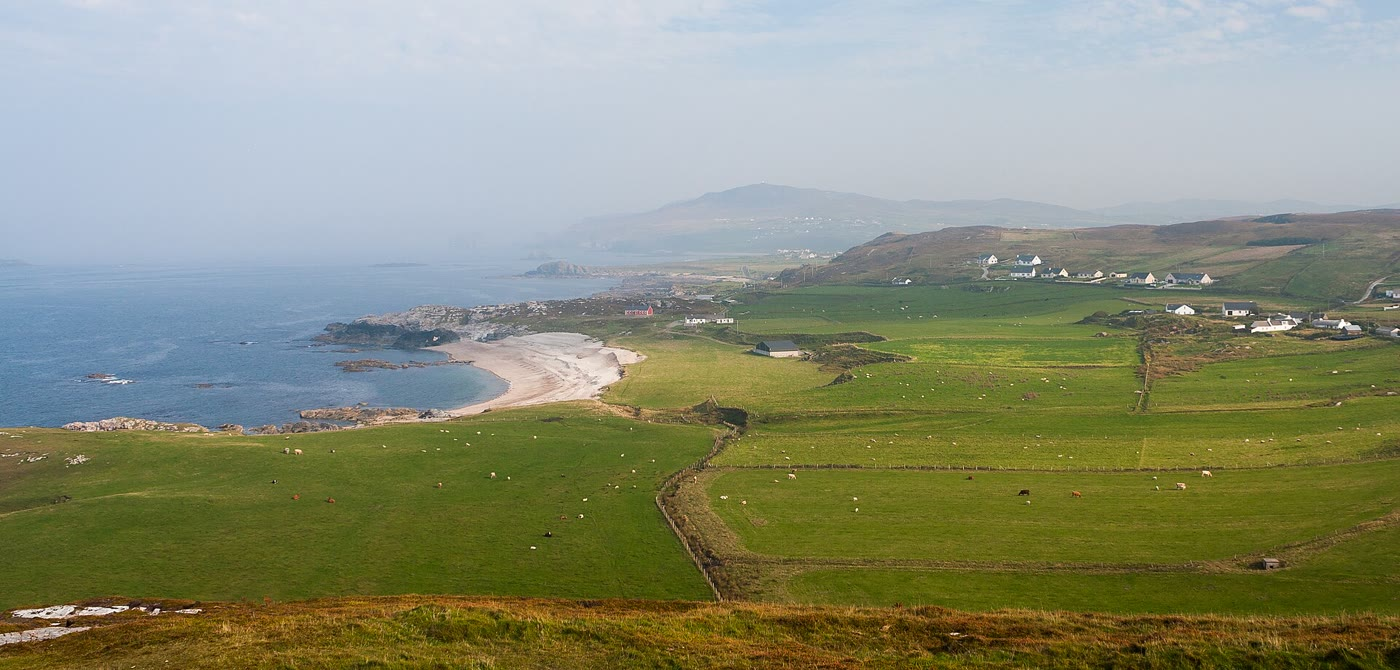
\includegraphics[width=\linewidth]{images/book5/b3-raised-beach-malin.jpg}

{\scriptsize De opgeheven stranden van Ballyhillin, Malin Head, in het noorden van
Ierland: ruggen van kiezels van oude kustlijnen, opgetild boven de zee toen het land
omhoogkwam nadat zijn ijskap was gesmolten. Foto A.~F.~Borchert, CC BY-SA 4.0.}
\end{minipage}
\end{inthefield}
% ledger: photo:b3-raised-beach

\section{Convectie over de hele mantel en de diepe structuur ervan}

Convecteert de mantel als één laag, of als twee, boven en onder de
discontinuïteit bij \qty{670}{km}? Tomografie (zie \cref{ch:b3:seismology-imaging})
geeft gedeeltelijk antwoord: sommige slabs vlakken af boven de discontinuïteit, andere
zinken erdoor de onderste mantel in, zodat massa de grens oversteekt en de twee lagen niet
van elkaar afgesloten. De toename van de viscositeit met de diepte laat de onderste
mantel trager stromen, en slabs vertragen en worden dikker bij het binnenkomen.

Aan de basis van de mantel toont tomografie twee brede gebieden met lage S-golfsnelheid,
onder Afrika en onder de Stille Oceaan, de grote
provincies met lage S-golfsnelheid (LLSVP's). Ze zijn waarschijnlijk chemisch verschillend van de mantel erboven
en dichter, eerder hopen dan hete pluimen. De grote magmatische provincies en
kimberlieten van de afgelopen paar honderd miljoen jaar barstten vooral uit boven hun
randen, alsof pluimen opstegen aan de randen van de hopen, waar de hete
thermische grenslaag aan de basis van de mantel wordt er tegenaan geveegd.
% ledger: st12:llsvp

\section{Oefeningen}

\begin{exercise}[$\star$]\label{exo:b3:mantle-convection:1}
Bereken het \omterm{def:b3:mantle-convection:rayleigh}{Rayleighgetal} van een bovenmantellaag van \qty{670}{km} dik met
$\rho = \qty{3500}{kg.m^{-3}}$, $g = \qty{9.9}{m.s^{-2}}$, $\alpha =
\qty{3e-5}{K^{-1}}$, $\Delta T = \qty{1000}{K}$, $\kappa =
\qty{e-6}{m^2.s^{-1}}$ en $\eta = \qty{5e20}{Pa.s}$. Hoeveel keer is het kritisch,
bij vrijglijdende randen?
\end{exercise}

\begin{exercise}[$\star$]\label{exo:b3:mantle-convection:2}
Bereken de \omterm{def:b3:mantle-convection:maxwell}{Maxwelltijd} van een mantel met viscositeit \qty{e21}{Pa.s} en
schuifmodulus \qty{7.7e10}{Pa}, in jaren. Reageert de mantel elastisch of
viscoos op het tweemaal per dag optredende aardgetij, op het smelten van een
ijskap, en op het zinken van een slab?
\end{exercise}

\begin{exercise}[$\star$]\label{exo:b3:mantle-convection:3}
Met $\eta = \qty{e21}{Pa.s}$, $\rho = \qty{3300}{kg.m^{-3}}$ en $g =
\qty{9.8}{m.s^{-2}}$, bereken de relaxatietijd van een uniforme halfruimte voor
belastingen met golflengte 1000 en \qty{3000}{km}. Welke herstelt sneller?
\end{exercise}

\begin{exercise}[$\star$]\label{exo:b3:mantle-convection:4}
Met $g = \qty{9.8}{m.s^{-2}}$, $\rho_m = \qty{3300}{kg.m^{-3}}$, $\rho_w =
\qty{1030}{kg.m^{-3}}$, $\alpha = \qty{3.1e-5}{K^{-1}}$, $T_m - T_0 =
\qty{1450}{K}$, $\kappa = \qty{0.8e-6}{m^2.s^{-1}}$ en \qty{1}{Myr} $=
\qty{3.156e13}{s}$, bereken de \omterm{prop:b3:mantle-convection:ridge-push}{rugduwkracht} bij \qty{50}{Myr}. Hoeveel
keer kleiner is het dan een slabtrek van \qty{4.6e13}{N.m^{-1}}?
\end{exercise}

\begin{exercise}[$\star\star$]\label{exo:b3:mantle-convection:5}
Een klomp mantelmateriaal van \qty{10}{km} breed, \qty{300}{K} warmer dan zijn
omgeving, stijgt met de snelheid $\rho g\alpha\Delta Td^2/\eta$ (neem $\rho =
\qty{3300}{kg.m^{-3}}$, $g = \qty{9.8}{m.s^{-2}}$, $\alpha = \qty{3e-5}{K^{-1}}$,
$\eta = \qty{e21}{Pa.s}$, $\kappa = \qty{e-6}{m^2.s^{-1}}$). (a) Bereken zijn
stijgtijd over zijn eigen grootte en zijn diffusietijd $d^2/\kappa$, en toon aan dat hun
verhouding zijn \omterm{def:b3:mantle-convection:rayleigh}{Rayleighgetal} is. (b) Stijgt hij of koelt hij eerst af? (c)
Hoe groot moet hij zijn opdat zijn \omterm{def:b3:mantle-convection:rayleigh}{Rayleighgetal} 657.5 bereikt?
\end{exercise}

\begin{exercise}[$\star\star$]\label{exo:b3:mantle-convection:6}
Voor een laag met een diepte van \qty{2891}{km} bij $\mathrm{Ra} = \num{e7}$, met $\kappa =
\qty{e-6}{m^2.s^{-1}}$, $k = \qty{3.1}{W.m^{-1}.K^{-1}}$, $\Delta T =
\qty{1450}{K}$ en $\mathrm{Ra}_c = 657.5$, bereken de
grenslaagdikte, het \omterm{def:b3:mantle-convection:nusselt}{Nusseltgetal}, de snelheidsschaal in \unit{cm/yr} en de
warmtestroom.
\end{exercise}

\begin{exercise}[$\star\star$]\label{exo:b3:mantle-convection:7}
Een verzonnen hotspotzwelling heeft een dwarsdoorsnede van \qty{8e8}{m^2} over
hotspotspoor, en de plaat erboven beweegt met \qty{9}{cm/yr}. Met $\rho_m - \rho_w =
\qty{2270}{kg.m^{-3}}$, bereken de drijfvermogenflux en de warmtestroom met $c_p =
\qty{1170}{J.kg^{-1}.K^{-1}}$ en $\alpha = \qty{3.1e-5}{K^{-1}}$. Welk deel
van de \qty{46.7}{TW} van de Aarde is het?
\end{exercise}

\begin{exercise}[$\star\star$]\label{exo:b3:mantle-convection:8}
Een pluimkop met een straal van \qty{400}{km}, lichter dan de mantel met
\qty{30}{kg.m^{-3}}, stijgt door een mantel met viscositeit \qty{e21}{Pa.s}. Met
de wet van Stokes, bereken zijn snelheid in \unit{m/yr} en de tijd die nodig is om
\qty{2000}{km} te stijgen.
\end{exercise}

\begin{exercise}[$\star\star$]\label{exo:b3:mantle-convection:9}
Een gebied werd met \qty{300}{m} neergedrukt toen zijn ijskap smolt, \qty{10}{kyr} geleden,
en relaxeert met $\tau = \qty{4.4}{kyr}$. Bereken de resterende indrukking vandaag en
de huidige opheffingssnelheid. Vergelijk met de \qty{10.3}{mm/yr} gemeten nabij
Umeå.
\end{exercise}

\begin{exercise}[$\star\star\star$]\label{exo:b3:mantle-convection:10}
(a) Toon aan de hand van de uitdrukking voor $F_{rp}$ in het bewijs van
\cref{prop:b3:mantle-convection:ridge-push}, toon aan dat de eerste term,
$\tfrac12(\rho_m - \rho_w)gw^2$, is de tweede term tussen de haken. (b) Toon aan dat
$\int_0^\infty x\operatorname{erfc}x\,\mathrm dx = 1/4$, door partieel te integreren.
(c) Bereken met de waarden van oefening 4 de twee termen bij \qty{100}{Myr}.
\end{exercise}

\begin{exercise}[$\star\star\star$]\label{exo:b3:mantle-convection:11}
Toon aan dat $f(k) = (\pi^2 + k^2)^3/k^2$ het kleinst is bij $k = \pi/\sqrt2$, waar
het gelijk is aan $27\pi^4/4$. Leid af de breedte van een paar convectiecellen bij
het ontstaan, in eenheden van $d$, en de breedte van één cel.
\end{exercise}

\begin{exercise}[$\star\star\star$]\label{exo:b3:mantle-convection:12}
Een plaat met een lengte van \qty{6000}{km} beweegt met \qty{6}{cm/yr} over een mantellaag
van \qty{150}{km} dik, met viscositeit \qty{e20}{Pa.s}, waarvan de basis in rust is. (a)
Bereken de \omterm{def:b3:mantle-convection:basal-drag}{basale weerstand} in \unit{MPa} en de weerstandskracht per eenheid van lengte van de plaat.
(b) Vergelijk met een rugduw van \qty{3.8e12}{N.m^{-1}} en een slabtrek van
\qty{4.6e13}{N.m^{-1}}. (c) Als één tiende van de slabtrek de plaat bereikt,
bij welke snelheid houdt de weerstand de aandrijvende krachten in evenwicht?
\end{exercise}

\section{Probleem: Herstel van Lake Ardo}

\begin{problem}[{Weekendprobleem --- het isostatisch herstel van een verzonnen meerbekken,
de viscositeit van de mantel eronder, en de convectie die die viscositeit
toelaat}]
\label{pb:b3:mantle-convection:1}
% values: calc/ch06.py; gia_relaxation.py, convection_scaling.py
Lake Ardo, een verzonnen meer, vulde een bekken van \qty{250}{km} breed, afgedamd door een
ijskap, en stond \qty{300}{m} diep gedurende ongeveer vijftigduizend jaar.
Veertienduizend jaar geleden brak de ijsdam door en liep het meer binnen enkele weken leeg.
Haar hoogste strandlijn, die bij het ontstaan horizontaal lag, is nu scheef; gedateerde strandlijnen van
de kleine meren die in het bekken zijn overgebleven, geven de opheffing van het centrum sinds de
afvoer, ten opzichte van de rand, die nauwelijks bewoog:

\smallskip
\begin{center}\small
\begin{tabular}{lcccccc}
\hline
tijd sinds de afvoer (kyr) & 1 & 2 & 4 & 6 & 9 & 14\\
opheffing van het centrum (m) & 11.5 & 21.6 & 38.0 & 50.5 & 64.0 & 77.2\\
\hline
\end{tabular}
\end{center}
\smallskip

Neem $\rho_w = \qty{1000}{kg.m^{-3}}$, $\rho_m = \qty{3300}{kg.m^{-3}}$, $g =
\qty{9.8}{m.s^{-2}}$, \qty{1}{yr} $= \qty{3.156e7}{s}$, en behandel de mantel als
een uniforme viskeuze halfruimte.

\medskip\noindent\textbf{Deel I --- De belasting.}
\begin{enumerate}
  \item Bereken de druk van het meer op de bodem.
  \item Bereken de indrukking van de bodem bij isostatisch evenwicht, en verklaar
        waarom de dichtheid van de mantel, en niet die van de korst, erin voorkomt.
  \item Behandel het meer als een schijf en bereken de massa van het water.
  \item Verklaar waarom de hoogste strandlijn nu scheef ligt, en bereken de
        gemiddelde helling van de rand naar het centrum, in meter per kilometer.
  \item De indrukking wordt behandeld als één harmonische, waarvan de ingedrukte helft, van
        $-\lambda/4$ tot $\lambda/4$, het meer overspant. Geef $\lambda$ en $k =
        2\pi/\lambda$.
  \item Over welke diepte neemt de stroming onder zo'n belasting af met een factor
        $e$?
\end{enumerate}

\medskip\noindent\textbf{Deel II --- De relaxatietijd.}
\begin{enumerate}[resume]
  \item Neem aan dat het meer evenwicht had bereikt, en bereken de indrukking die
        op elk tijdstip uit de tabel overblijft.
  \item Toon aan dat, als de indrukking exponentieel vervalt, haar logaritme
        lineair met de tijd daalt.
  \item Bereken $\tau$ uit de tijdstippen 1 en \qty{14}{kyr}.
  \item Voorspel de opheffing op \qty{6}{kyr} met die $\tau$ en vergelijk met de
        tabel.
  \item Bereken de indrukking die vandaag overblijft en de huidige opheffingssnelheid van het
        centrum, in \unit{mm/yr}.
  \item Hoeveel opheffing volgt er nog?
  \item Hoeveel jaar nog duurt het voordat de opheffingssnelheid onder
        \qty{0.5}{mm/yr} zakt?
\end{enumerate}

\medskip\noindent\textbf{Deel III --- De viscositeit.}
\begin{enumerate}[resume]
  \item Bereken de viscositeit van de halfruimte uit $\tau$.
  \item Vergelijk die met de viscositeiten van de bovenmantel van \num{3.4e20} tot
        \qty{1e21}{Pa.s}, die onder Fennoscandië zijn gevonden. Welk deel van de mantel
        bemonstert het herstel van Lake Ardo?
  \item Bereken met die viscositeit de relaxatietijd van een belasting
        met een golflengte van \qty{3000}{km}. Waarom zou een echte ijskap van die grootte
        langzamer ontspannen dan hier?
  \item Wat doet een elastische lithosfeer, hier buiten beschouwing gelaten, met het herstel van een
        belasting van slechts \qty{250}{km} breed?
  \item Bereken de \omterm{def:b3:mantle-convection:maxwell}{Maxwelltijd} van de mantel met $\mu = \qty{7.7e10}{Pa}$,
        en verklaar of een viskeus model gerechtvaardigd was.
  \item Controleer de aanname van vraag 7: welk deel van de evenwichtsindrukking
        werd bereikt terwijl het meer bestond?
  \item Hoeveel zou $\log_{10}\eta$ veranderen als $\lambda$ gelijk wordt gesteld aan
        \qty{250}{km}?
\end{enumerate}

\medskip\noindent\textbf{Deel IV --- Convectie.} Neem een bovenmantellaag
\qty{670}{km} diep met $\rho = \qty{3700}{kg.m^{-3}}$, $g =
\qty{9.9}{m.s^{-2}}$, $\alpha = \qty{3.1e-5}{K^{-1}}$, $\Delta T =
\qty{1450}{K}$, $\kappa = \qty{e-6}{m^2.s^{-1}}$, $k = \qty{3.1}{W.m^{-1}.K^{-1}}$
en de viscositeit van Deel III.
\begin{enumerate}[resume]
  \item Bereken het \omterm{def:b3:mantle-convection:rayleigh}{Rayleighgetal} van de laag.
  \item Hoeveel keer de kritische waarde is dat ($\mathrm{Ra}_c = 657.5$)?
  \item Bereken de dikte van de grenslaag en het \omterm{def:b3:mantle-convection:nusselt}{Nusseltgetal}.
  \item Bereken de snelheidsschaal in \unit{cm/yr} en vergelijk met de plaatsnelheden
        van 1 tot \qty{7.5}{cm/yr}.
  \item Bereken de warmtestroom en geef twee redenen waarom die achterblijft bij het
        gemiddelde van de Aarde, \qty{92}{mW.m^{-2}}.
  \item Geef de viscositeit van de bovenmantel onder Lake Ardo als $\log_{10}$ van
        $\eta$ in \unit{Pa.s}.
\end{enumerate}
\end{problem}
